\documentclass{article}[12pt]

\usepackage[francais]{babel}
\usepackage{boxedminipage}
\usepackage[utf8]{inputenc}
\usepackage{amsfonts,amssymb,amsmath}
\usepackage[pdftex]{graphicx}
\usepackage{vmargin}

\usepackage{todonotes}
\setpapersize{A4}
\setmarginsrb{2cm}{2cm}{2cm}{2cm}{0cm}{0cm}{0cm}{0cm} 

\setlength{\parindent}{0pt}

%\setlength{\textwidth}{17cm}
%\setlength{\evensidemargin}{0pt}
%\setlength{\oddsidemargin}{0pt}
%\setlength{\topmargin}{0pt}


\begin{document}
\begin{center}
\framebox[1.07\width]{
\begin{minipage}[b]{4cm}
%\includegraphics[width=4.5cm]{LOGO_EM.pdf}  
\end{minipage} 
\begin{minipage}[b]{11cm}
\ \\[.1cm]
%%%%%%%%%%%%%%%%%%%
%   ANNÉE 
Année 2021-2022
%%%%%%%%%%%%%%%%%%%
\hspace{\stretch{1}} 
%%%%%%%%%%%%%%%%%%%
% NUMERO DE SESSION
$1^\textrm{ère}$ session 
%%%%%%%%%%%%%%%%%%%
\\[.15cm]
\begin{center}
%%%%%%%%%%%%%%%%%%%
% DONNÉES DU MODULE
\textsc{Algorithmique et Structures de données}\\
\textsc{IF111}\\
\textsc{Rohan Fossé}\\
%%%%%%%%%%%%%%%%%%%
\end{center}
\ \\[.2cm]
%%%%%%%%%%%%%%%%%%%
% Données diverses
Filière : {T\'el\'ecom}
\hspace{\stretch{1}}
Année : {2021 - 2022}
\hspace{\stretch{1}}
Semestre : {1}
\\[.2cm]
Date de l'examen : {18 Janvier 2022}
\hspace{\stretch{1}}
Durée de l'examen : {2h}
%%%%%%%%%%%%%%%%%%%
\\[.2cm]
\begin{tabular}{llll}
%%%%%%%%%%%%%%%%%%%
% remplacer $\Box$ par $\boxtimes$ pour cocher.
Documents autorisés &  $\Box$     & %\hspace{.5cm} &
sans document & $\boxtimes$ \\
Calculatrice autorisée & $\Box$ &
non autorisée & $\boxtimes$ \\
% remplacer $\Box$ par $\boxtimes$ pour cocher.
\end{tabular}
\\[.2cm]
%Autre : {.......}
\\[.2cm]
\end{minipage}
}

\end{center}

\vspace{1cm}
\begin{center}\huge{\textbf{SUJET}}\end{center}
\vspace{1cm}

%%%%%%%%%%%%%%%%%%%
% DÉBUT DU SUJET
%%%%%%%%%%%%%%%%%%%

\begin{center}
  \begin{boxedminipage}{\linewidth}
    {\large {\bf Nom et Prénom} :}~\\
  \end{boxedminipage}
\end{center}

\textbf{
\begin{itemize}
\item Toutes les parties du sujet sont indépendantes (en particulier les exercices) ;
\item Il est impératif de répondre dans les espaces prévus à cet effet : ce qui dépasse
  ne sera pas lu. Pour les parties où il faut écrire du code, merci d'écrire une ligne
  devant chaque numéro. \textbf{Vous êtes donc limités dans la quantité de code que vous êtes
  autorisés à écrire pour chaque question.}
\item Merci d'écrire dans un français correct : orthographe, grammaire et conjugaison
  seront pris en compte dans la correction ;
\item Vos codes doivent être indentés correctement ;
\item Le barême est donné à titre indicatif ;
\item Merci de retirer les pages d'annexe du sujet avant de rendre votre copie ;
\item Enfin, n'oubliez pas d'indiquer votre NOM sur la copie !
\end{itemize}
}

\section*{Exercice 1}
On considère le code suivant. On cherche à mesurer la
complexité dans le pire cas en fonction de n. Pour cela, on utilise la variable compteur, qui est incrémentée à
chaque passage dans le « tant que » interne.

\begin{figure}[h!]
    \centering
    \hspace*{-9cm}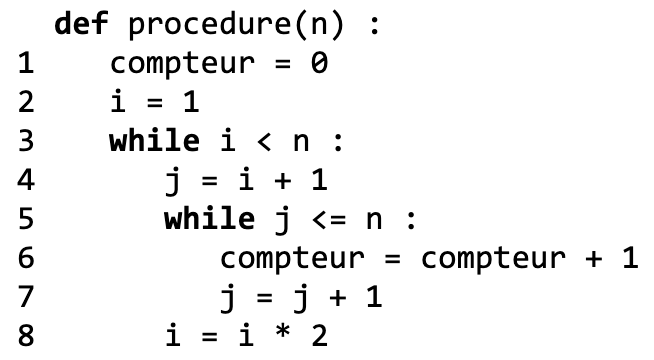
\includegraphics[scale=0.6]{procedure.png}
    \label{fig:my_label}
\end{figure}

\begin{enumerate}
    \item Quelle est la valeur finale du compteur dans le cas où n = 16 ?
    \item Considérons le cas particulier où n est une puissance de 2 : on suppose que $n = 2^p$ avec p connu.
Quelle est la valeur finale du compteur en fonction de p ? Justifiez votre réponse.
    \item Exprimez le résultat précédent en fonction de n.
    \item En conclure la complexité dans le pire des cas, en notation $\mathcal{O}$, de cette procédure
\end{enumerate}


\section*{Exercice 2}
\begin{enumerate}


    \item Donner la suite de fibonacci sous forme d'équations de récurrence
    
    \item Écrire la fonction de fibonacci sous forme récursive. 
    
    \item L'écrire sous forme terminale récursive
\end{enumerate}


\section*{Exercice 3}

Soit la liste de clés L = (5, 17, 12, 19, 6, 23, 34, 1). Pour chacune des structures suivantes, en partant d’un arbre binaire vide, vous devez dessiner l’arbre après chacune des insertions des éléments de la liste L.
    \begin{enumerate}
        \item Arbre binaire de recherche (ABR)
        \item Tas min
        \item Tas max
    \end{enumerate}

\section*{Exercice 4}



 Le tableau ci-dessous représente le réseau routier d'un pays. Les sommets A, B, C, D, E, F et G désignent des villes. Une case du tableau représente la distance entre deux villes.
 
 \begin{figure}[h!]
    \centering
    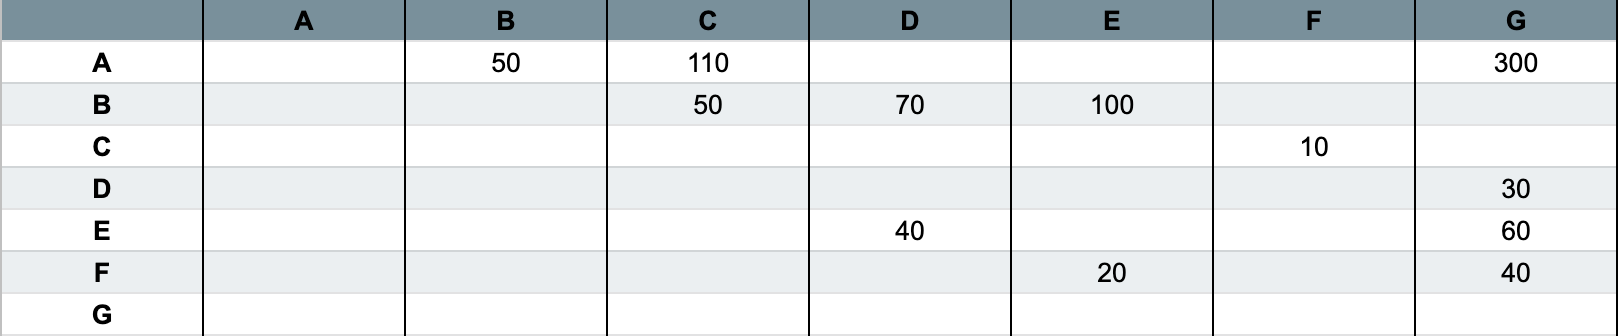
\includegraphics[scale=0.5]{table_graph.png}
    \label{fig:my_label}
\end{figure}

 
 Par exemple, le tableau signifie qu'il existe une route allant de A à B de 50 km (mais pas de route allant de B à A).\\
 
 A l'aide d'un graphe, proposer un trajet de distance minimale permettant d'aller de la ville A à la ville G.\\




 On s'intéresse dorénavant au même graphe mais \underline{non orienté} et \underline{non pondéré}.\\
 Répondre aux questions suivantes :
\begin{enumerate}
    \item Ce graphe est-il connexe ?
    \item Ce graphe est-il complet ?
    \item Ce graphe admet-il une chaîne eulérienne ?
    \item Ce graphe admet-il un cycle eulérien ?
    \item Quel est la taille de la plus grande clique de ce graphe ?
    \item Déterminer, en justifiant, le nombre chromatique de ce graphe.
\end{enumerate}


\section*{Exercice 5}
Écrivez les fonctions suivantes sur les piles.
\begin{enumerate}
    \item $plus\_souvent(x,y,p)$ qui renvoie $True$ si l’élément $x$ apparaît plus de fois que l’élément $y$ dans la pile $p$ et $False$ sinon;
    \item $millieme(p)$ qui renvoie le millième élément de la pile $p$ (on suppose que la pile p a au moins
mille éléments donc il n’est pas nécessaire de traiter le cas d’erreur);
    \item $facto\_pile(p)$ qui renvoie la pile contenant la factorielle de chacun des éléments de la pile $p$
(si p contient les valeurs 4, 3 et 2, la fonction doit renvoyer une pile contenant les valeurs 24, 6 et
2) ;
    \item $produit(p_1,p_2)$ qui renvoie la pile contenant les produits des éléments de $p_1$ et $p_2$, que l’on
suppose être de même longueur (si $p_1$ contient les entiers 1, 2 et 4 et $p_2$ contient les entiers 2, 3 et
4, la fonction doit renvoyer une pile contenant les valeurs 2, 6 et 16) ;
    \item $double(p)$ qui renvoie True si chaque élément de la pile est supérieur au double de son prédécesseur, et $False$ sinon (par exemple sur la pile 2, 5, 10 et 23 la fonction renverra $True$ mais sur la pile 2, 4, 9, 12 et 25 elle renverra $False$ car 12 est inférieur au double de 9) ;
\end{enumerate}
Pour toute pile $P$, vous avez à disposition les opérations de base suivantes pour la manipuler : \texttt{EstVide(P)},  \texttt{Empiler(P,e)}, \texttt{Depiler(P)} et \texttt{Sommet(P)}.


\end{document}

